%%% Template originaly created by Karol Kozioł (mail@karol-koziol.net) and modified for ShareLaTeX use

\documentclass[a4paper,11pt]{article}

\usepackage[T1]{fontenc}
\usepackage[utf8]{inputenc}
\usepackage{graphicx}
\usepackage{xcolor}

\renewcommand\familydefault{\sfdefault}
\usepackage{tgheros}
\usepackage[defaultmono]{droidmono}

\usepackage{amsmath,amssymb,amsthm,textcomp}
\usepackage{enumerate}
\usepackage{multicol}
\usepackage{tikz}
\usetikzlibrary{bayesnet}
\usepackage[bb=boondox]{mathalfa}

\usepackage{geometry}
\geometry{total={210mm,297mm},
left=25mm,right=25mm,%
bindingoffset=0mm, top=20mm,bottom=20mm}

\usepackage{natbib}

\linespread{1.3}

\newcommand{\linia}{\rule{\linewidth}{0.5pt}}

% custom theorems if needed
\newtheoremstyle{mytheor}
    {1ex}{1ex}{\normalfont}{0pt}{\scshape}{.}{1ex}
    {{\thmname{#1 }}{\thmnumber{#2}}{\thmnote{ (#3)}}}

\theoremstyle{mytheor}
\newtheorem{defi}{Definition}

% my own titles
\makeatletter
\renewcommand{\maketitle}{
\begin{center}
\vspace{2ex}
{\huge \textsc{\@title}}
\vspace{1ex}
\\
\linia\\
\@author \hfill \@date
\vspace{4ex}
\end{center}
}
\makeatother
%%%

% custom footers and headers
\usepackage{fancyhdr}
\pagestyle{fancy}
\lhead{}
\chead{}
\rhead{}
\lfoot{Assignment \textnumero{} 1}
\cfoot{}
\rfoot{Page \thepage}
\renewcommand{\headrulewidth}{0pt}
\renewcommand{\footrulewidth}{0pt}
%sections
\renewcommand\thesection{\arabic{section}}
\renewcommand\thesubsection{\thesection.\alph{subsection}}

%

% code listing settings
\usepackage{listings}
\lstset{
    language=Python,
    basicstyle=\ttfamily\small,
    aboveskip={1.0\baselineskip},
    belowskip={1.0\baselineskip},
    columns=fixed,
    extendedchars=true,
    breaklines=true,
    tabsize=4,
    prebreak=\raisebox{0ex}[0ex][0ex]{\ensuremath{\hookleftarrow}},
    frame=lines,
    showtabs=false,
    showspaces=false,
    showstringspaces=false,
    keywordstyle=\color[rgb]{0.627,0.126,0.941},
    commentstyle=\color[rgb]{0.133,0.545,0.133},
    stringstyle=\color[rgb]{01,0,0},
    numbers=left,
    numberstyle=\small,
    stepnumber=1,
    numbersep=10pt,
    captionpos=t,
    escapeinside={\%*}{*)}
}

%%%----------%%%----------%%%----------%%%----------%%%

\usepackage{caption}
\usepackage{subcaption}
\usepackage{bm}

\newcommand{\E}{\Bbb{E}}

\newcommand{\Var}{\mathrm{Var}}

\newcommand{\Cov}{\mathrm{Cov}}

\newcommand*\diff{\mathop{}\!\mathrm{d}}

\newcommand*\Diff[1]{\mathop{}\!\mathrm{d^#1}}

\begin{document}

\title{Probabilistic Modelling and Reasoning \textnumero{} 1}

\author{Georgi Tinchev, s1549117, The University of Edinburgh}

\date{07/03/2016}

\maketitle

\section{Question 1: Player skill graphical models}


\subsection{}

\begin{figure}[htpb!]
    \centering
    \tikz{ %
        \node[obs] (r1) {$r^1$} ; %
        \node[latent, above=of r1, yshift=0.5cm, xshift=-1cm] (s1) {$s_1$} ; %
        \node[latent, above=of r1, yshift=0.5cm, xshift=0.7cm] (s2) {$s_2$} ; %
        \node[obs, xshift=1.5cm] (r2) {$r^2$};
        \node[latent, right=of s2] (s3) {$s_3$};
        \factor[above=of r1, yshift=0.2cm] {r1-factor} {$\mathcal{\eta}$} {} {};
        \factor[above=of r2, yshift=0.2cm] {r2-factor} {$\mathcal{\mu}$} {} {};
        \node[obs, yshift=4.5cm, xshift=0.7cm] (r3) {$r^3$};
        \factor[below=of r3, yshift=-0.4cm, xshift=0cm] {r3-factor} {$\mathcal{\phi}$} {} {};
        \edge {s1,s2} {r1-factor} ; %
        \edge{s2,s3} {r2-factor};
        \edge{s1,s3} {r3-factor};
        \factoredge {} {r1-factor} {r1} ; %
        \factoredge {} {r2-factor} {r2} ; %
        \factoredge {} {r3-factor} {r3} ; %
    }
    \caption{Factor graph of simple player skill model when observing three games between three players. The games are denoted as the factors $\phi$, $\mu$ and $\eta$. Game outcomes are denoted as $r^{(k)}$, where $k\in{\{1,2,3\}}$ being the different games played. The result of the games, denoted $r^{(k)}\in{\{0,1\}}$ with 0 indicating a loss and 1 indicating a win. The players' skills are identified as $s_1$, $s_2$ and $s_3$, where the index denotes the ID of the player $\in{\{1,2,3\}}$ respectively.}
    \label{fig:fg}
\end{figure}
      
\subsection{}
\subsubsection{$I(s_1,s_2|r^{(2)})$}
\label{sec:first_indep}
There are 2 paths leading from $s_1$ to $s_2$, namely $s_1-\eta-s_2$ and $s_1-\phi-s_3-\mu-s_2$. The former path is blocked, as $\eta$ has two incoming edges and neither $\eta$, nor $r^{(1)}$ (being all descendants) are in the conditioning set (being $r^{(2)}$). The latter is also blocked, but the case is slightly more complicated. Firstly, $\mu$ has two incoming edges, however, its descendant is in the conditioning set ($r^{(2)}$), therefore, the path is not blocked there. Secondly, $\phi$ also has two incoming edges and neither $\phi$, nor $r^{(3)}$ are in the conditioning set, therefore, the path is blocked there.
Thus, as the two paths are blocked $=> I(s_1,s_2|r^{(2)})$.
\subsubsection{$I(s_1,s_2|r^{(2)},r^{(3)})$}
As identified in Section~\ref{sec:first_indep}, there are 2 paths. The path $s_1-\eta-s_2$ is still blocked, as $\eta$, nor any of its descendants are in the conditioning set. The path $s_1-\phi-s_3-\mu-s_2$, however, is now unblocked, as for all factors and variables with 2 incoming edges, there is a child that belongs to the conditioning set, namely $r^{(3)}$ is a child of $\phi$ and $r^{(2)}$ is a child of $\mu$, both of them being in the conditioning set. Therefore, $s_1,s_2$ are conditionally dependent on the set $\{r^{(2)},r^{(3)}\}$.
\subsection{}
\begin{figure}[htpb!]
    \centering
    \tikz{ %
        \node[obs] (r1) {$r^1$} ; %
        
        \node[latent, right=of r1] (s2) {$s_2$} ; %
        \node[obs, right=of s2] (r2) {$r^2$};
        \node[latent, above=of s2, xshift=-1cm] (s1) {$s_1$} ; %
        \node[latent, above=of s2, xshift=1cm] (s3) {$s_3$} ; %
        \node[obs, above=of s2, yshift=1.5cm] (r3) {$r^3$};
        
        \edge[-] {s1,s2} {r1,s3} ; %
        \edge[-] {s2,s3} {r2,s1};
        \edge[-] {s1,s3} {r3,s2};
        
    }
    \caption{Markov network of simple player skill model when observing three games between three players. The observed and latent variables are denoted in a similar way, as Figure~\ref{fig:fg}. Game outcomes are denoted as $r^{(k)}$, where $k\in{\{1,2,3\}}$ being the different games played. The result of the games, denoted $r^{(k)}\in{\{0,1\}}$ with 0 indicating a loss and 1 indicating a win. The players' skills are identified as $s_1$, $s_2$ and $s_3$, where the index denotes the ID of the player $\in{\{1,2,3\}}$ respectively.}
    \label{fig:mn}
\end{figure}

\subsection{}
\label{sec:1d}

In order to avoid repetition I will use two indices, namely, $i$, $j$, $k$, where $i \neq j \neq k$. Equation~\ref{eq:ci_1d} and~\ref{eq:ci_1d_2} generalise the conditional independence statements in Figure~\ref{fig:mn}. Also, the following rules must hold: $s_i, s_j \in ne(r^{(i)}) || s_i, s_j \in ne(r^{(j)})$ for Equation~\ref{eq:ci_1d} and $s_i, s_j \in ne(r^{(i)})$ for Equation~\ref{eq:ci_1d_2}.

\begin{equation}
    \label{eq:ci_1d}
    I(r^{(i)}, r^{(j)} |s_i,s_j,\{s_k, r^{(k)}\})
\end{equation}

\begin{equation}
    \label{eq:ci_1d_2}
    I(r^{(i)}, s_k | s_i,s_j,\{r^{(j)}, r^{(k)}\})
\end{equation}

The set in the conditioning part of Equation~\ref{eq:ci_1d} means that including any combination or no combination of the elements inside the set would still work.

There are no conditional independence statements between the variables $s_1$, $s_2$, $s_3$, as disregarding how many $r$ and $s$ variables we remove, due to the u-separation rule, we cannot make them conditionally independent.

In other words, the games are only dependent on the players that play them.

\section{Question 2: Gaussian player skill model}
\label{sec:2}
\subsection{}
From the figure, one can express the joint probability distribution as follows:

\begin{equation}
    \label{eq:joint_distr}
    p(p_b,p_w,s_b,s_w) = \frac{1}{Z}\phi_{1}(p_w)\phi_{2}(s_w,p_w)\phi_{3}(s_b)\phi_{4}(s_b,p_b)\phi_{5}(p_w,p_b,r)
\end{equation}

Thereafter, using chain rule, $p(p_b,p_w|s_b,s_w)$ can be expressed as follows:
\begin{equation}
    \label{eq:chain_rule}
    p(p_b,p_w|s_b,s_w) = \frac{p(p_b,p_w,s_b,s_w)}{p(s_b,s_w)} = \frac{p(p_b,p_w,s_b,s_w)}{\int_{p_b,p_w} p(p_b,p_w,s_b,s_w)}= 
\end{equation}

\begin{equation}
    \label{eq:chain_rule_1}
    \frac{\frac{1}{Z}\phi_{1}(s_w)\phi_{2}(s_w,p_w)\phi_{3}(s_b)\phi_{4}(s_b,p_b)\phi_{5}(p_w,p_b,r)}{\int_{p_b,p_w}\frac{1}{Z}\phi_{1}(s_w)\phi_{2}(s_w,p_w)\phi_{3}(s_b)\phi_{4}(s_b,p_b)\phi_{5}(p_w,p_b,r)}
\end{equation}

\begin{equation}
    \label{eq:chain_rule_2}
    \frac{\frac{1}{Z}\phi_{1}(p_w)\phi_{2}(s_w,p_w)\phi_{3}(p_b)\phi_{4}(s_b,p_b)\phi_{5}(p_w,p_b,r)}{\frac{1}{Z}\phi_{1}(p_w)\phi_{3}(p_b)\int_{p_b,p_w}\phi_{2}(s_w,p_w)\phi_{4}(s_b,p_b)\phi_{5}(p_w,p_b,r)}
\end{equation}

\begin{equation}
    \label{eq:chain_rule_3}
    \frac{\phi_{2}(s_w,p_w)\phi_{4}(s_b,p_b)\phi_{5}(p_w,p_b,r)}{\int_{p_b,p_w}\phi_{2}(s_w,p_w)\phi_{4}(s_b,p_b)\phi_{5}(p_w,p_b,r)}
\end{equation}

\begin{equation}
    \label{eq:chain_rule_4}
    \frac{\phi_{2}(s_w,p_w)\phi_{4}(s_b,p_b)}{\int_{p_b,p_w}\phi_{2}(s_w,p_w)\phi_{4}(s_b,p_b)}
\end{equation}

\begin{equation}
    \label{eq:chain_rule_5}
    \phi_{2}(s_w,p_w)\phi_{4}(s_b,p_b)
\end{equation}

\subsection{}
% for E[theta]
\subsubsection{$\E[\theta \mid s_b,s_w]$}

\begin{equation}
    \label{e_theta}
    \Bbb{E}[\theta\mid s_w,s_b] = \frac{1}{\sqrt{2}\beta}\Bbb{E}[(p_w-s_w)+(p_b-s_b) \mid s_w,s_b]
\end{equation}

\begin{equation}
    \label{e_theta_2}
    \frac{1}{\sqrt{2}\beta} \Bigg( \Bbb{E}[p_w+p_b \mid s_w,s_b]-s_w-s_b \Bigg)
\end{equation}

\begin{equation}
    \label{e_theta_3}
    \frac{1}{\sqrt{2}\beta} \Bigg( \Bbb{E}[p_w\mid s_w,s_b] + \Bbb{E}[p_b \mid s_w,s_b]-s_w-s_b \Bigg)
\end{equation}


\begin{equation}
    \label{e_theta_4}
    \frac{1}{\sqrt{2}\beta} \Bigg( s_w+s_b-s_w-s_b \Bigg) = 0
\end{equation}

% for E[psi]
\subsubsection{$\E[\psi \mid s_b,s_w]$}

\begin{equation}
    \label{e_psi}
    \Bbb{E}[\psi\mid s_w,s_b] = \frac{1}{\sqrt{2}\beta}\Bbb{E}[(p_w-s_w)-(p_b-s_b) \mid s_w,s_b]
\end{equation}

\begin{equation}
    \label{e_psi_2}
    \frac{1}{\sqrt{2}\beta} \Bigg( \Bbb{E}[p_w-p_b \mid s_w,s_b]-s_w+s_b \Bigg)
\end{equation}

\begin{equation}
    \label{e_psi_3}
    \frac{1}{\sqrt{2}\beta} \Bigg( \Bbb{E}[p_w\mid s_w,s_b] - \Bbb{E}[p_b \mid s_w,s_b]-s_w+s_b \Bigg)
\end{equation}


\begin{equation}
    \label{e_psi_4}
    \frac{1}{\sqrt{2}\beta} \Bigg( s_w-s_b-s_w+s_b \Bigg) = 0
\end{equation}


% for E[theta^2]
\subsubsection{$\E[\theta^2 \mid s_b,s_w]$}

\begin{equation}
    \label{e_theta_sq}
    \Bbb{E}[\theta^2\mid s_w,s_b] = \frac{1}{2\beta^2}\Bbb{E}[((p_w-s_w)+(p_b-s_b))^2 \mid s_w,s_b]
\end{equation}

\begin{equation}
    \label{e_theta_sq_2}
    \frac{1}{2\beta^2} \Bigg( \underbrace{\Bbb{E}[(p_w-s_w)^2\mid s_w,s_b]}_\text{A} + \underbrace{2\Bbb{E}[(p_w-s_w)(p_b-s_b)\mid s_w,s_b]}_\text{B} + \underbrace{\Bbb{E}[(p_b-s_b)^2\mid s_w,s_b]}_\text{C} \Bigg)
\end{equation}

\begin{equation}
    \label{e_theta_sq_2_a}
    A=\Bbb{E}[p_w^2\mid s_w,s_b] - 2s_w\Bbb{E}[p_w\mid s_w,s_b] + s_{w}^{2}
\end{equation}

\begin{equation}
    \label{e_theta_sq_2_a_1}
    A=\Var(p_w)+\E[p_w\mid s_w,s_b]^2 - 2s_w^2 + s_{w}^{2} = \Var(p_w) = \beta^2
\end{equation}

\begin{equation}
    \label{e_theta_sq_2_b}
    B=2\E[p_bp_w \mid s_w,s_b] - 2s_b\E[p_w \mid s_w,s_b] - 2s_w\E[p_b \mid s_w,s_b] + 2s_bs_w
\end{equation}

\begin{equation}
    \label{e_theta_sq_2_b_1}
    B=2 \Bigg( \E[p_b \mid s_w,s_b]\E[p_w \mid s_w,s_b] + \Cov(p_b,p_w) \Bigg) - 2s_bs_w - 2s_ws_b + 2s_bs_w
\end{equation}

\begin{equation}
    \label{e_theta_sq_2_b_2}
    B=2 \Bigg( \E[p_b \mid s_w,s_b]\E[p_w \mid s_w,s_b] + \Cov(p_b,p_w) \Bigg) - 2s_bs_w
\end{equation}

\begin{equation}
    \label{e_theta_sq_2_b_2}
    B=2 \Bigg( s_bs_w +  \underbrace{\Cov(p_b,p_w)}_\text{$p_w$ and $p_b$ are CI $=> \Cov(p_w,p_b)=0$} \Bigg) - 2s_bs_w=0
\end{equation}

\begin{equation}
    \label{e_theta_sq_2_c}
    C=\Bbb{E}[p_b^2\mid s_w,s_b] - 2s_b\Bbb{E}[p_b\mid s_w,s_b] + s_{b}^{2}
\end{equation}

\begin{equation}
    \label{e_theta_sq_2_c_1}
    C=\Var(p_b)+\E[p_b\mid s_w,s_b]^2 - 2s_b^2 + s_{b}^{2} = \Var(p_b) = \beta^2
\end{equation}

From Equation~\ref{e_theta_sq_2}:

\begin{equation}
    \label{e_theta_sq_all_combined}
    \frac{1}{2\beta^2}(A+B+C)=\frac{\beta^2+0+\beta^2}{2\beta^2} = 1
\end{equation}

% for psi^2
\subsubsection{$\E[\psi^2 \mid s_b,s_w]$}

\begin{equation}
    \label{e_psi_sq}
    \Bbb{E}[\psi^2\mid s_w,s_b] = \frac{1}{2\beta^2}\Bbb{E}[((p_w-s_w)-(p_b-s_b))^2 \mid s_w,s_b]
\end{equation}

\begin{equation}
    \label{e_psi_sq_2}
    \frac{1}{2\beta^2} \Bigg( \underbrace{\Bbb{E}[(p_w-s_w)^2\mid s_w,s_b]}_\text{D} - \underbrace{2\Bbb{E}[(p_w-s_w)(p_b-s_b)\mid s_w,s_b]}_\text{E} + \underbrace{\Bbb{E}[(p_b-s_b)^2\mid s_w,s_b]}_\text{F} \Bigg)
\end{equation}

\begin{equation}
    \label{e_psi_sq_2_a}
    D=\Bbb{E}[p_w^2\mid s_w,s_b] - 2s_w\Bbb{E}[p_w\mid s_w,s_b] + s_{w}^{2}
\end{equation}

\begin{equation}
    \label{e_psi_sq_2_a_1}
    D=\Var(p_w)+\E[p_w\mid s_w,s_b]^2 - 2s_w^2 + s_{w}^{2} = \Var(p_w) = \beta^2
\end{equation}

\begin{equation}
    \label{e_psi_sq_2_b}
    E=2\E[p_bp_w \mid s_w,s_b] - 2s_b\E[p_w \mid s_w,s_b] - 2s_w\E[p_b \mid s_w,s_b] + 2s_bs_w
\end{equation}

\begin{equation}
    \label{e_psi_sq_2_b_1}
    E=2 \Bigg( \E[p_b \mid s_w,s_b]\E[p_w \mid s_w,s_b] + \Cov(p_b,p_w) \Bigg) - 2s_bs_w - 2s_ws_b + 2s_bs_w
\end{equation}

\begin{equation}
    \label{e_psi_sq_2_b_2}
    E=2 \Bigg( \E[p_b \mid s_w,s_b]\E[p_w \mid s_w,s_b] + \Cov(p_b,p_w) \Bigg) - 2s_bs_w
\end{equation}

\begin{equation}
    \label{e_psi_sq_2_b_2}
    E=2 \Bigg( s_b s_w +  \underbrace{\Cov(p_b,p_w)}_\text{$p_w$ and $p_b$ are CI $=> \Cov(p_w,p_b)=0$} \Bigg) - 2s_bs_w=0
\end{equation}

\begin{equation}
    \label{e_psi_sq_2_c}
    F=\Bbb{E}[p_b^2\mid s_w,s_b] - 2s_b\Bbb{E}[p_b\mid s_w,s_b] + s_{b}^{2}
\end{equation}

\begin{equation}
    \label{e_psi_sq_2_c_1}
    F=\Var(p_b)+\E[p_b\mid s_w,s_b]^2 - 2s_b^2 + s_{b}^{2} = \Var(p_b) = \beta^2
\end{equation}

From Equation~\ref{e_psi_sq_2}:

\begin{equation}
    \label{e_psi_sq_all_combined}
    \frac{1}{2\beta^2}(D-E+F)=\frac{\beta^2-0+\beta^2}{2\beta^2} = 1
\end{equation}

\subsubsection{$\E[\psi\theta \mid s_b,s_w]$}

\begin{equation}
    \label{e_psi_theta}
    \Bbb{E}[\psi\theta\mid s_w,s_b] = \frac{1}{2\beta^2}\Bbb{E}[(p_w-s_w)^2-(p_w-s_w)(p_b-s_b)+(p_w-s_w)(p_b-s_b)-(p_b-s_b)^2 \mid s_w,s_b]
\end{equation}

\begin{equation}
    \label{e_psi_theta_1}
    \Bbb{E}[\psi\theta\mid s_w,s_b] = \frac{1}{2\beta^2}\Bbb{E}[(p_w-s_w)^2-(p_w-s_w)(p_b-s_b)+(p_w-s_w)(p_b-s_b)-(p_b-s_b)^2 \mid s_w,s_b]
\end{equation}

\begin{equation}
    \label{e_psi_theta_2}
    \Bbb{E}[\psi\theta\mid s_w,s_b] = \frac{1}{2\beta^2} \Bigg( \underbrace{\Bbb{E}[(p_w-s_w)^2 \mid s_w,s_b]}_\text{G} - \underbrace{\E[(p_b-s_b)^2 \mid s_w,s_b]}_\text{H} \Bigg)
\end{equation}

\begin{equation}
    \label{e_psi_theta_3}
    G=\Bbb{E}[p_w^2\mid s_w,s_b] - 2s_w\Bbb{E}[p_w\mid s_w,s_b] + s_{w}^{2}
\end{equation}

\begin{equation}
    \label{e_psi_theta_4}
    G=\Var(p_w)+\E[p_w\mid s_w,s_b]^2 - 2s_w^2 + s_{w}^{2} = \Var(p_w) = \beta^2
\end{equation}

\begin{equation}
    \label{e_psi_theta_5}
    H=\Bbb{E}[p_b^2\mid s_w,s_b] - 2s_b\Bbb{E}[p_b\mid s_w,s_b] + s_{b}^{2}
\end{equation}

\begin{equation}
    \label{e_psi_theta_6}
    H=\Var(p_b)+\E[p_b\mid s_w,s_b]^2 - 2s_b^2 + s_{b}^{2} = \Var(p_b) = \beta^2
\end{equation}

From Equation~\ref{e_psi_theta_2}:

\begin{equation}
    \label{e_psi_theta_7}
    G-H= \frac{\beta^2-\beta^2}{2\beta^2}=0
\end{equation}

\subsubsection{$\mathbb{p}[\theta,\psi \mid s_b,s_w]$}

$\mathbb{p}(\theta|s_b,s_w)$ is a distribution, however, as it is composed of $p_w$, $p_b$, $s_w$, $s_b$, that are all Gaussian distributions, $\mathbb{p}(\theta|s_b,s_w)$ is also a Gaussian distribution. Its mean($\E[\theta|s_b,s_w]$) is 0 and its variance is 1 ($\E[\theta^2|s_b,s_w]$), therefore, $\mathbb{p}(\theta|s_b,s_w)$ is a standard normal Gaussian distribution.

$\mathbb{p}(\psi|s_b,s_w)$ is a distribution, however, as it is composed of $p_w$, $p_b$, $s_w$, $s_b$, that are all Gaussian distributions, $\mathbb{p}(\psi|s_b,s_w)$ is also a Gaussian distribution. Its mean($\E[\psi|s_b,s_w]$) is 0 and its variance is 1 ($\E[\psi^2|s_b,s_w]$), therefore, $\mathbb{p}(\psi|s_b,s_w)$ is a standard normal Gaussian distribution.

Based on the 2 aforementioned statements, the joint distribution $\mathbb{p}(\theta,\psi|s_b,s_w)$ is a joint standard multivariate Gaussian distribution, expressed as follows:

\begin{equation}
    \label{p_psi_theta}
    \mathbb{p}(\theta,\psi|s_b,s_w)= \frac{1}{\sqrt{(2\pi)^2\mid\Sigma\mid}}exp \Bigg( -\frac{1}{2}(x-\mu)^T\Sigma^{-1}(x-\mu) \Bigg)
\end{equation}

With the following $x$, $\mu$ and $\Sigma$:

\begin{align}
    \label{vec_theta_psi}
    x &= \begin{bmatrix}
           \theta \\
           \psi \\
         \end{bmatrix}
\end{align}

\begin{align}
    \label{vec_theta_psi_mean}
    \mu &= \begin{bmatrix}
           \E[\theta \mid s_b,s_w] \\
           \E[\psi \mid s_b,s_w] \\
         \end{bmatrix} = \begin{bmatrix}
                            0 \\
                            0 \\
                          \end{bmatrix}
\end{align}

\begin{align}
    \label{vec_theta_psi_cov_mat}
    \Sigma &= \begin{bmatrix}
           \Var(\theta) & \Cov(\theta,\psi)\\
           \Cov(\theta,\psi) & \Var(\psi) \\
         \end{bmatrix} = \begin{bmatrix}
                            1 & 0 \\
                            0 & 1 \\
                          \end{bmatrix}
\end{align}

The $\Cov[\theta,\psi \mid s_b,s_w]=0$ as $\E[\psi\theta \mid s_b,s_w]=0$, $\E[\psi \mid s_b,s_w]=0$ and $\E[\theta \mid s_b,s_w]=0$ , meaning that $\theta$ and $\psi$ are independent.

Leading to the following form:
  
\begin{equation}
    \label{p_psi_theta}
    \mathbb{p}(\theta,\psi|s_b,s_w)= \frac{1}{2\pi}\exp \Big( -\frac{1}{2}(\theta^2+\psi^2) \Big)
\end{equation}

In order to prove this result one could use the change of variable.

Firstly express $p_b$ and $p_w$ in terms of $\psi$ and $\theta$.

\begin{equation}
    \label{p_b_in_psi}
    p_b = -\sqrt{2}\beta\psi + p_w - s_w + s_b
\end{equation}

\begin{equation}
    \label{p_w_in_theta}
    p_w = \sqrt{2}\beta\theta + s_w - p_b + s_b
\end{equation}

Substituting Equation~\ref{p_b_in_psi} in Equation~\ref{p_w_in_theta} results in:

\begin{equation}
    \label{p_b_in_p_w}
    p_w = \sqrt{2}\beta\theta + s_w + \sqrt{2}\beta\psi - p_w + s_w - s_b + s_b
\end{equation}

\begin{equation}
    \label{p_b_in_p_w_2}
    p_w = \frac{\sqrt{2}\beta(\theta+\psi) + 2s_w}{2}
\end{equation}

Substituting Equation~\ref{p_w_in_theta} in Equation~\ref{p_b_in_psi} results in:

\begin{equation}
    \label{p_w_in_p_b}
    p_b = -\sqrt{2}\beta\psi + \sqrt{2}\beta\theta + s_w - p_b + s_b - s_w + s_b
\end{equation}

\begin{equation}
    \label{p_w_in_p_b_2}
    p_b = \frac{\sqrt{2}\beta(\theta-\psi) + 2s_b}{2}
\end{equation}

Substituting the factors for their values in Equation~\ref{eq:chain_rule_5}, we get the following:

\begin{equation}
    \label{p_w_in_p_b_full_gaussian}
    p(p_b,p_w|s_b,s_w) = \mathcal{N}(p_b)\mathcal{N}(p_w) = 
\end{equation}

\begin{equation}
    \label{p_w_in_p_b_full_gaussian_2}
    \frac{1}{{\beta \sqrt {2\pi } }}e^{{{ - \left( {p_b - s_b } \right)^2 } \mathord{\left/ {\vphantom {{ - \left( {p_b - s_b } \right)^2 } {2\beta ^2 }}} \right. \kern-\nulldelimiterspace} {2\beta ^2 }}}
    \frac{1}{{\beta \sqrt {2\pi } }}e^{{{ - \left( {p_w - s_w } \right)^2 } \mathord{\left/ {\vphantom {{ - \left( {p_w - s_w } \right)^2 } {2\beta ^2 }}} \right. \kern-\nulldelimiterspace} {2\beta ^2 }}}
\end{equation}

In order to change the variable, we would have to compute the derivative of a 2x2 Jacobian matrix given below:

\begin{equation}
    \label{eq:jacobian}
    J = \begin{bmatrix}
            \frac{\partial p_w}{\partial \theta} & \frac{\partial p_b}{\partial \theta}\\
            \frac{\partial p_w}{\partial \psi} & \frac{\partial p_b}{\partial \psi}\\ 
        \end{bmatrix} = 
        \begin{bmatrix}
            \frac{\sqrt{2}\beta}{2} & \frac{\sqrt{2}\beta}{2}\\
            \frac{\sqrt{2}\beta}{2}& -\frac{\sqrt{2}\beta}{2}\\
        \end{bmatrix}
\end{equation}

The absolute value of the derivative derivative is equal to:

\begin{equation}
    \label{eq:jac_drv}
   \lvert \det(J) \rvert = \left\lvert\frac{\partial p_w}{\partial \theta}\frac{\partial p_b}{\partial \psi} - \frac{\partial p_b}{\partial \theta}\frac{\partial p_w}{\partial \psi} \right\rvert = \left\lvert\frac{\sqrt{2}\beta}{2}\Big(-\frac{\sqrt{2}\beta}{2}\Big) - \frac{\sqrt{2}\beta}{2}\frac{\sqrt{2}\beta}{2} \right\rvert = \left\lvert-\frac{2\beta^2}{4} - \frac{2\beta^2}{4} \right\rvert = \left\lvert-\beta^2\right\rvert = \beta^2
\end{equation}

Now we can express $p(p_b,p_w|s_b,s_w)$ as $p(\theta,\psi|s_b,s_w)$, when substituting $p_w$ and $p_b$ from Equation~\ref{p_b_in_p_w_2} and~\ref{p_w_in_p_b_2} in Equation~\ref{p_w_in_p_b_full_gaussian_2} and multiplying by the absolute value of the derivative of the Jacobian, expressed in Equation~\ref{eq:jac_drv}.

\begin{equation}
    \label{p_w_in_p_b_full_gaussian_2}
    \int\int\frac{1}{{\beta \sqrt {2\pi } }}e^{{{ - \left( {\frac{\sqrt{2}\beta}{2}(\theta-\psi) + s_b - s_b } \right)^2 } \mathord{\left/ {\vphantom {{ - \left( {\frac{\sqrt{2}\beta}{2}(\theta-\psi) + s_b - s_b } \right)^2 } {2\beta ^2 }}} \right. \kern-\nulldelimiterspace} {2\beta ^2 }}}
    \frac{1}{{\beta \sqrt {2\pi } }}e^{{{ - \left( {\frac{\sqrt{2}\beta}{2}(\theta+\psi) + s_w - s_w } \right)^2 } \mathord{\left/ {\vphantom {{ - \left( {\frac{\sqrt{2}\beta}{2}(\theta+\psi) + s_w - s_w } \right)^2 } {2\beta ^2 }}} \right. \kern-\nulldelimiterspace} {2\beta ^2 }}} \lvert \det(J) \rvert\diff\theta\diff\psi
\end{equation}

\begin{equation}
    \label{p_w_in_p_b_full_gaussian_3}
    \int\int\frac{1}{{2\pi\beta^2}}
    e^{-\frac{\beta^2}{2\beta^2}\left( {\frac{1}{2}(\theta-\psi)^2} + \frac{1}{2}(\theta+\psi)^2 \right) } \beta^2\diff\theta\diff\psi=
\end{equation}

\begin{equation}
    \label{p_w_in_p_b_full_gaussian_4}
    \int\int\frac{1}{{2\pi}}
    e^{-\frac{1}{2}\left( \theta^2-\theta\psi +\theta\psi+\psi^2 \right) } \diff\theta\diff\psi
\end{equation}

\begin{equation}
    \label{p_w_in_p_b_full_gaussian_5}
    p(\theta,\psi|s_b,s_w) = \frac{1}{{2\pi}}
    e^{-\frac{1}{2}\left( \theta^2+\psi^2 \right) }
\end{equation}

\subsection{}
We can express the inequality $p(r=1|p_b,p_w)$ as follows:
\begin{equation}
    \label{int_p_w_p_b_0}
    \mathbb{1}[p_b > p_w]
\end{equation}

Using the change of variable from Equation~\ref{p_b_in_p_w_2} and~\ref{p_w_in_p_b_2}:

\begin{equation}
    \label{int_p_w_p_b_0}
    \frac{\sqrt{2}\beta(\theta-\psi) + 2s_b}{2} - \frac{\sqrt{2}\beta(\theta+\psi) + 2s_w}{2} > 0
\end{equation}

\begin{equation}
    \label{p_w_and_p_b_in_r_2}
    \sqrt{2}\beta(\theta-\psi) + 2s_b - \sqrt{2}\beta(\theta+\psi) + 2s_w > 0
\end{equation}

\begin{equation}
    \label{p_w_and_p_b_in_r_3}
    -\sqrt{2}\beta\psi + 2s_b - \sqrt{2}\beta\theta + 2s_w > 0
\end{equation}

\begin{equation}
    \label{p_w_and_p_b_in_r_4}
    2s_b + 2s_w > 2\sqrt{2}\beta\psi
\end{equation}

\begin{equation}
    \label{p_w_and_p_b_in_r_5}
    \mathbb{P}(r=1|\theta,\psi,s_b,s_w)=\mathbb{1}\Big[\frac{s_b + s_w}{\sqrt{2}\beta} > \psi\Big]
\end{equation}

\subsection{}

\begin{equation}
    \mathbb{P}(r=1|s_b,s_w) = \frac{\mathbb{P}(r=1,s_b,s_w)}{\mathbb{P}(s_b,s_w)}
\end{equation}

\begin{equation}
    \mathbb{P}(r=1|s_b,s_w) = \frac{\int_{\theta,\psi} \mathbb{P}(r=1,\theta,\psi,s_b,s_w)\diff{\theta}\diff{\psi}}{\mathbb{P}(s_b,s_w)}
\end{equation}

\begin{equation}
    \mathbb{P}(r=1|s_b,s_w) = \frac{\int_{\theta,\psi} \mathbb{P}(r=1|\theta,\psi,s_b,s_w)\mathbb{P}(\theta,\psi,s_b,s_w)\diff{\theta}\diff{\psi}}{\mathbb{P}(s_b,s_w)}
\end{equation}

\begin{equation}
    \mathbb{P}(r=1|s_b,s_w) = \frac{\mathbb{P}(s_b,s_w)\int_{\theta,\psi} \mathbb{P}(r=1|\theta,\psi,s_b,s_w)\mathbb{P}(\theta,\psi|s_b,s_w)\diff{\theta}\diff{\psi}}{\mathbb{P}(s_b,s_w)}
\end{equation}

Substituting Equation~\ref{p_w_and_p_b_in_r_5}, and splitting $p(\theta,\psi \mid s_b,s_w)$, as they are conditionally independent ($\E[\psi\theta \mid s_b,s_w]=0$, $\E[\theta \mid s_b,s_w]=0$, $\E[\psi \mid s_b,s_w]=0$, therefore, $\Cov(\psi,\theta)=0$), we get:

\begin{equation}
    \mathbb{P}(r=1|s_b,s_w) = \int_{\psi} \mathbb{1}\Big[\frac{s_b+s_w}{\sqrt{2}\beta}>\psi\Big]\mathbb{P}(\psi|s_b,s_w)\diff{\psi}\underbrace{\int_{\theta}\mathbb{p}(\theta|s_b,s_w)\diff{\theta}}_\text{1}
\end{equation}

Also, as $\mathbb{P}(\psi|s_b,s_w)$ has mean of $0$ and variance of $1$, we can model it as such:

\begin{equation}
    \label{eq:r_one_cdf}
    \mathbb{P}(r=1|s_b,s_w) = \int \mathbb{1}\Big[\frac{s_b+s_w}{\sqrt{2}\beta}>\psi\Big]\mathcal{N}( \psi ; 0,1 )\diff{\psi} = \Phi\Big[ \frac{s_b-s_w}{\sqrt{2}\beta} \Big]
\end{equation}

\subsection{}
In order for a game to be observed it has to be either won by the black player or by the white player. Here, I am ignoring the fact that it could be draw, as described in the assignment sheet. Thus, we can mathematically model this as follows:

\begin{equation}
    \label{eq:r_sum}
    \mathbb{P}(r|s_b,s_w) = \mathop{I}(r=1)\mathbb{P}(r=1|s_b,s_w) + \mathop{I}(r=0)\mathbb{P}(r=0|s_b,s_w)
\end{equation}

As this is a Bernoulli distribution, we can express $\mathbb{P}(r=0|s_b,s_w)$ as:

\begin{equation}
    \label{eq:r_zero_expression}
    \mathbb{P}(r=0|s_b,s_w) = 1 - \mathbb{P}(r=1|s_b,s_w)
\end{equation}

Substituting the result from Equation~\ref{eq:r_one_cdf} in Equation~\ref{eq:r_zero_expression}:

\begin{equation}
    \label{eq:r_zero_expression_2}
    \mathbb{P}(r=0|s_b,s_w) = 1 - \Phi\Big[ \frac{s_b-s_w}{\sqrt{2}\beta} \Big]
\end{equation}

Therefore, substituting Equation~\ref{eq:r_zero_expression_2} and~\ref{eq:r_one_cdf} in Equation~\ref{eq:r_sum}:

\begin{equation}
    \label{eq:r_sum_2}
    \mathbb{P}(r|s_b,s_w) = \mathop{I}(r=1)\Phi\Big[ \frac{s_b-s_w}{\sqrt{2}\beta} \Big] + \mathop{I}(r=0)\Big( 1-\Phi\Big[ \frac{s_b-s_w}{\sqrt{2}\beta} \Big] \Big)
\end{equation}

The above result is derived for one game. Based on Section~\ref{sec:1d}, I assume that each observed game is independently and identically distributed. I.e. each game does not depend in any way on other games, but only on the two players that play it, thus the expression can be rewritten as follows:

\begin{equation}
    \label{eq:r_iid}
    \mathbb{P} \Big[ \{r^{(k)}\}_{k=1}^{N}  \mid \{s_i\}_{i=1}^{M} \Big] = \prod_{k=1}^{N}\Big[
    \mathop{I}(r^{(k)}=1)\Phi\Big[ \frac{s_b-s_w}{\sqrt{2}\beta} \Big] + 
    \mathop{I}(r^{(k)}=0)\Big( 1-\Phi\Big[ \frac{s_b-s_w}{\sqrt{2}\beta} \Big] \Big)
    \Big]
\end{equation}

\subsection{}
\label{sec:2f}

Adopting Bayes Rule, we can rewrite the equation in the following fashion:

\begin{equation}
    \label{eq:2_f_bayes}
    \mathbb{P} \Big[ \{s_i\}_{i=1}^{M} \mid \{r^{(k)}\}_{k=1}^{N} \Big] = 
    \frac{\mathbb{P} \Big[ \{r^{(k)}\}_{k=1}^{N}  \mid \{s_i\}_{i=1}^{M} \Big]\mathbb{p} \Big[ \{s_i\}_{i=1}^{M} \Big]}
    {\mathbb{p} \Big[ \{r^{(k)}\}_{k=1}^{N} \Big]}
\end{equation}

\begin{equation}
    \label{eq:2_f_bayes_2}
    \mathbb{P} \Big[ \{s_i\}_{i=1}^{M} \mid \{r^{(k)}\}_{k=1}^{N} \Big] \propto \mathbb{P} \Big[ \{r^{(k)}\}_{k=1}^{N}  \mid \{s_i\}_{i=1}^{M} \Big]\mathbb{p} \Big[ \{s_i\}_{i=1}^{M} \Big]
\end{equation}

Taking into account the equality $1-\Phi(x)=\Phi(-x)$, we can rewrite Equation~\ref{eq:r_iid} as such:

\begin{equation}
    \label{eq:r_iid_2}
    \prod_{k=1}^{N}\Big[
    \mathop{I}(r^{(k)}=1)\Phi\Big[ \frac{s_b-s_w}{\sqrt{2}\beta} \Big] + 
    \mathop{I}(r^{(k)}=0)\Big(\Phi\Big[ \frac{s_w-s_b}{\sqrt{2}\beta} \Big] \Big)
    \Big]
\end{equation}

When $r^{(k)}=1$, the black player is the winner, similarly, when $r^{(k)}=1$, the white player is the winner, thus one can notice that the winner is always on the left of the equation, and the loser is always on the right. In other words, if we present the winner's skill as $s_{winner}$ and the loser's skill as $s_{loser}$, we can express the relations as follows:

\begin{equation}
    \label{eq:winner_loser}
    s_{winner}-s_{loser} = (s_b-s_w)^{(1-r^{(k)})}
\end{equation}

Thus, we can rewrite Equation~\ref{eq:r_iid_2} as follows:

\begin{equation}
    \label{eq:r_iid_3}
    \prod_{k=1}^{N}\Big[
    \mathop{I}(r^{(k)}=1)\Phi\Big[ \frac{s_{winner}-s_{loser}}{\sqrt{2}\beta} \Big] + 
    \mathop{I}(r^{(k)}=0)\Big(\Phi\Big[ \frac{s_{winner}-s_{loser}}{\sqrt{2}\beta} \Big] \Big)
    \Big]
\end{equation}

\begin{equation}
    \label{eq:r_iid_4}
    \prod_{k=1}^{N}\Big[
        \Phi\Big[ \frac{(s_{winner}-s_{loser})}{\sqrt{2}\beta} \Big]
        \Big(\mathop{I}(r^{(k)}=1) + \mathop{I}(r^{(k)}=0)\Big)
    \Big]
\end{equation}

As the sum of the two indicator functions will always produce 1, thus, we can rewrite Equation~\ref{eq:r_iid} as follows:

\begin{equation}
    \label{eq:r_iid_5}
    \mathbb{P} \Big[ \{r^{(k)}\}_{k=1}^{N}  \mid \{s_i\}_{i=1}^{M} \Big] = 
    \prod_{k=1}^{N}\Big[
        \Phi\Big[ \frac{s_{winner}-s_{loser}}{\sqrt{2}\beta} \Big]
    \Big]
\end{equation}

We can model the relation between $s_{winner}$ and $s_{loser}$ in terms of vectors. As we presented their relationship in Equation~\ref{eq:winner_loser}, it can also be expressed as a product of two vectors, namely $\bm{s}$ and $\bm{x^{(k)}}$. More specifically, $s$ will contain all the M player skills. While $\bm{x^{(k)}}$ will be a zero vector of magnitude M, where the winning player's skill will be substituted by $1$ and the losing player's skill by $-1$. For instance, if $M=30$ (number of players), players $2$ and $28$ play a game, and we want to calculate the probability of $2$ winning, then we would write it as $s=[0,0,1,....,-1,0]^T$. This model, however, does not account for the which player plays which colour, neither it accounts for $komi$ points. As the player's standard deviation ($\beta$), is constant in the model, we can include it in the $\bm{x^{(k)}}$ vector. Therefore, instead of $1$ and $-1$ we can write $\frac{1}{\sqrt{2}\beta}$ and $-\frac{1}{\sqrt{2}\beta}$ respectively. Thus, using the new notation, we can rewrite Equation~\ref{eq:r_iid_5} as follows:

\begin{equation}
    \label{eq:r_iid_6}
    \mathbb{P} \Big[ \{r^{(k)}\}_{k=1}^{N}  \mid \{s_i\}_{i=1}^{M} \Big] = 
    \prod_{k=1}^{N}\Big[
        \Phi[s^Tx^{(k)}]
    \Big]
\end{equation}

We can model the prior ($\mathbb{p} \Big[ \{s_i\}_{i=1}^{M} \Big]$), in matrix notation as well - $\mathcal{N}(s, m_0, V_0)$. As all players' skills has been initialised to have mean of 0, thus $m_0$ will be a vector of $0$s. Every player will has a variance of $\sigma^2$, thus we can model $V_0$ as a diagonal matrix with $\sigma^2$ on the main diagonal.

\begin{equation}
    \label{eq:V_0}
    V_0 = \begin{bmatrix}
            \sigma^2 &  0  & \ldots & 0\\
            0  &  \sigma^2 & \ldots & 0\\
            \vdots & \vdots & \ddots & \vdots\\
            0  &   0       &\ldots & \sigma^2
           \end{bmatrix}
\end{equation}

Substituting the likelihood, Equation~\ref{eq:r_iid_6}, in Equation~\ref{eq:2_f_bayes_2}, and the prior for players' skills, we get:

\begin{equation}
    \label{eq:2f_final}
    \mathbb{P} \Big[ \{s_i\}_{i=1}^{M} \mid \{r^{(k)}\}_{k=1}^{N} \Big] \propto
    \prod_{k=1}^{N}\Big[
        \Phi[s^Tx^{(k)}]
    \Big]
    \mathcal{N}(s, m_0, V_0)
\end{equation}

\section{Approximate inference with Go game data}
\label{sec:3}

\subsection{}
In order to interpret the graphs, I will firstly illustrate the process of expectation propagation with messages, passing through the graph, given in Figure 2 of the assignment sheet, which copy is presented at Figure~\ref{fig:fig_2_assignment}. There, the flow of messages for only one game of Go are shown and are labelled in red and blue. Further, I will associate some of the messages with the different plots and explain what they represent.
\begin{figure}[htpb!]
    \centering
    \tikz{ %
        \node[obs] (r1) {$r^{(1)}$} ; %
        \node[latent, left=of r1, yshift=0.9cm, xshift=-0.7cm] (pw) {$p_w$} ; %
        \node[latent, left=of r1, below=of pw] (pb) {$p_b$} ; %
        \factor[left=of r1, xshift=-0.2cm] {r1-factor} {} {} {};
        \edge[color=red] {pw} {r1-factor} ; %
        \edge[color=blue] {r1-factor} {pb} ; %
        \edge[color=red] {r1} {r1-factor}; %
        \factor[left=of pw, xshift=-.6cm] {pw-factor} {below:$\mathcal{N}(p_w;s_w,\beta^2)$} {} {};
        \factor[left=of pb, xshift=-.6cm] {pb-factor} {above:$\mathcal{N}(p_b;s_b,\beta^2)$} {} {};
        \node[latent, left=of pw, xshift=-1.2cm] (sw) {$s_w$} ; %
        \node[latent, left=of pb, xshift=-1.2cm] (sb) {$s_b$} ; %
        \edge[color=red] {sw} {pw-factor} ; %
        \edge[color=blue] {pb-factor} {sb} ; %
        \edge[color=red] {pw-factor} {pw} ; %
        \edge[color=blue] {pb} {pb-factor} ; %
        \factor[left=of sw, xshift=-1.2cm] {sw-factor} {left:$\mathcal{N}(s_w;0,\sigma^2)$} {} {};
        \factor[left=of sb, xshift=-1.2cm] {sb-factor} {left:$\mathcal{N}(s_b;0,\sigma^2)$} {} {};
        \edge[color=red] {sw-factor} {sw} ; %
        \edge[color=red] {sb-factor} {sb} ; %
        \node[const, left=of r1-factor, xshift=-3cm]  (beta) {$\beta$} ; %
        \node[const, left=of beta, xshift=-2cm]  (alpha) {$\alpha$} ; %
        \edge[dotted] {beta} {pb-factor} ; %
        \edge[dotted] {beta} {pw-factor} ; %
        \edge[dotted] {alpha} {sb-factor} ; %
        \edge[dotted] {alpha} {sw-factor} ; %
        \draw node [above=of alpha, fill=white, xshift=2cm] {\textcolor{red}{(1)}};
        \draw node [above=of alpha, fill=white, xshift=3.9cm] {\textcolor{red}{(2)}};
        \draw node [above=of alpha, fill=white, xshift=5.1cm] {\textcolor{red}{(3)}};
        \draw node [above=of alpha, fill=white, xshift=7cm, yshift=-0.5cm] {\textcolor{red}{(4)}};
        \draw node [above=of alpha, fill=white, xshift=7.7cm, yshift=-1cm] {\textcolor{red}{(5)}};
        \draw node [above=of alpha, fill=white, xshift=7cm, yshift=-2.3cm] {\textcolor{blue}{(6)}};
        \draw node [above=of alpha, fill=white, xshift=5.1cm, yshift=-2.7cm] {\textcolor{blue}{(7)}};
        \draw node [above=of alpha, fill=white, xshift=3.9cm, yshift=-2.7cm] {\textcolor{blue}{(8)}};
        \draw node [above=of alpha, fill=white, xshift=2cm, yshift=-2.7cm] {\textcolor{red}{(9)}};
    }
    \caption{Factor graph of Gaussian player skill model for a single game. The variables $r^{(1)}$, $s_b$ and $s_w$ are as defined for Figure~\ref{fig:fg}. The variables $p_b$ and $p_w$ are the performances of the black and white player respectively in the game. The red edges are the original messages, where as the blue edges are the approximated ones for each individual factor locally.}
    \label{fig:fig_2_assignment}
\end{figure}

On Figure~\ref{fig:fig_2_assignment}, message $(1)$ is only a Gaussian ($\mathcal{N}(s_w;0,\sigma^2)$) from the factor on the left. Message $(2)$ is a product of the all connected factors to the variable $s_w$, which in this case is only 1 - the Gaussian, therefore, it is just a copy of that Gaussian. In order to calculate message $(3)$, we have to multiply the output from message $(2)$ with the factor $\mathcal{N}(p_w;s_w,\beta^2)$ and integrate over $s_w$. This convolution could be estimated exactly~\cite[Equation 2.115]{bishop2006pattern} and produces another Gaussian distribution. Message $(4)$ is a copy of message $(3)$, as it represents the product of all incoming messages, which in this case is only the output from $(3)$. Message $(5)$ is a Bernoulli distribution. To compute message $(6)$, we have to product messages $(4)$ and $(5)$, integrate over $p_w$ and sum over $r^{(1)}$. If we consider the case, where black are the winners, i.e. $r^{(1)}=1 \Leftrightarrow \mathbb{1}[p_b > p_w]$, then message $(5)$ becomes 1, similarly it becomes 0, when $r^{(1)}=0 \Leftrightarrow \mathbb{1}[p_w \geq p_b]$. From this, we can deduct that the regions. where $p_w$ is winning will be multiplied by 0~\cite{bishop2013model}. Finally, when we integrate over $p_w$, we receive the true factor, showed in green on Figure~\ref{fig:diag_from_orig}.

\begin{figure}[htpb!]
    \centering
    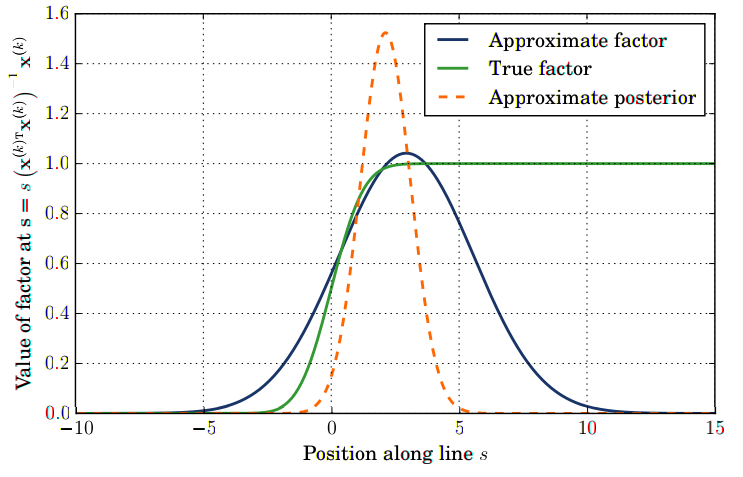
\includegraphics[scale=0.5]{diag_from_ass}
    \caption{Values of corresponding approximate and true factors and scaled value of approximate posterior density along line $s=s|x^{(k)}|^{-1}x^{(k)}$ for a single factor in the diagonal covariance approximate densities.}
    \label{fig:diag_from_orig}
\end{figure}

This is the case, as for each value of $p_b$, a "cut" Gaussian (area being 0, due to $r^{(1)}=0$) is being integrated, which results in the Cumulative Density Function of a Gaussian (shown in green on Figure~\ref{fig:diag_from_orig})~\cite{bishop2013model}. As the true factor has mean and variance of infinity (CDF), we cannot simply approximate it. As we want the approximation to be local, i.e. at each factor, we need to retrieve an approximate factor, which is in fact the message on the same edge $(6)$, but in the opposite direction, from $p_b$ to the factor~\cite{bishop2013model}. This will be a Gaussian, passed from $(9)-(8)-(7)-(6)$ in the same fashion as messages $(1)-...-(4)$, previously discussed. I will denote this message as context($c_k$)~\cite{bishop2013model}, which will help me outline the relationship between the green and blue plots. The true factor will be denoted as $f_t$. The factor approximation is denoted as $f_a$. The messages can be visualised on Figure~\ref{fig:cumGaus_msgs}.

\begin{figure}[htpb!]
    \centering
    \begin{subfigure}[b]{0.3\textwidth}
        \centering
        \tikz{ %
            \node[obs] (r1) {$r^{(1)}$} ; %
            \node[latent, left=of r1, yshift=0.9cm, xshift=-0.7cm] (pw) {$p_w$} ; %
            \node[latent, left=of r1, below=of pw] (pb) {$p_b$} ; %
            \factor[left=of r1, xshift=-0.2cm] {r1-factor} {} {} {};
            \edge {pw} {r1-factor} ; %
            \edge[color=gray] {pb} {r1-factor} ; %
            \edge {r1-factor} {r1}; %
            \draw node [right=of pb, fill=white, xshift=-0.7cm, yshift=0.1cm] {\textcolor{gray}{$c_k$}};
        }
        \caption{$c_k$}
        \label{fig:msgs_a}
    \end{subfigure}
    ~
    \begin{subfigure}[b]{0.3\textwidth}
        \centering
        \tikz{ %
            \node[obs] (r1) {$r^{(1)}$} ; %
            \node[latent, left=of r1, yshift=0.9cm, xshift=-0.7cm] (pw) {$p_w$} ; %
            \node[latent, left=of r1, below=of pw] (pb) {$p_b$} ; %
            \factor[left=of r1, xshift=-0.2cm] {r1-factor} {} {} {};
            \edge {pw} {r1-factor} ; %
            \edge[color=green] {r1-factor} {pb} ; %
            \edge {r1} {r1-factor}; %
            \draw node [right=of pb, fill=white, xshift=-0.7cm, yshift=0.1cm] {\textcolor{green}{$f_t$}};
        }
        \caption{$\Phi(s^Tx^{(k)})$}
        \label{fig:msgs_b}
    \end{subfigure}
    ~
    \begin{subfigure}[b]{0.3\textwidth}
        \centering
        \tikz{ %
            \node[obs] (r1) {$r^{(1)}$} ; %
            \node[latent, left=of r1, yshift=0.9cm, xshift=-0.7cm] (pw) {$p_w$} ; %
            \node[latent, left=of r1, below=of pw] (pb) {$p_b$} ; %
            \factor[left=of r1, xshift=-0.2cm] {r1-factor} {} {} {};
            \edge {pw} {r1-factor} ; %
            \edge[color=blue] {r1-factor} {pb} ; %
            \edge {r1} {r1-factor}; %
            \draw node [right=of pb, fill=white, xshift=-0.7cm, yshift=0.1cm] {\textcolor{blue}{$f_a$}};
        }
        \caption{$\mathcal{N}(s;m_k,V_k)$}
        \label{fig:msgs_c}
    \end{subfigure}
    \caption{Message passing during EP, colour coded to match Figure~\ref{fig:diag_from_orig}.}
    \label{fig:cumGaus_msgs}
\end{figure}

What we are trying to achieve is to get from the CDF in Figure~\ref{fig:msgs_b} to the Gaussian in Figure~\ref{fig:msgs_c}.
The approximation can be mathematically expressed as follows:

\begin{equation}
    \label{eq:ge_eq_proj_ce}
    c_kf_a = approx(f_tc_k)
\end{equation}

Multiplying the true factor($f_t$) with context message($c_k$) will give us the true marginal. However, their product will not be a Gaussian, but it will still have a finite mean and variance. Thus, we can simply create a Gaussian distribution with the same mean and variance ($approx$ function), resulting in:

\begin{equation}
    \label{eq:approx_gaus}
    \mathcal{N}(x;\E[f_tc_k];\Var(f_tc_k))
\end{equation}

Finally, we can substitute this new distribution in Equation~\ref{eq:ge_eq_proj_ce}, in order to retrieve the final result for the blue factor approximation:

\begin{equation}
    \label{eq:g_eq_proj_ce_div_c}
    c_kf_a = \mathcal{N}(x;\E[f_tc_k];\Var(f_tc_k))=c_k\mathcal{N}(s;m_k,V_k)
\end{equation}

Now if we divide by the context message ($c_k$), we will receive the factor approximation, denoted as message $(6)$ in Figure~\ref{fig:fig_2_assignment}.

Continuing with the messages in Figure~\ref{fig:fig_2_assignment}, now that we have that the message approximation $(6)$ is a Gaussian, message $(7)$ is just a copy of it, but it also differs from its original message, that was supposed to be a normal CDF. Message $(8)$ is again a convolution of two Gaussians - the factor and the message, which results in a Gaussian. Also, please note that message $(8)$ is also different from its original message. 

Now we can now calculate the approximate posterior for the black player ($s_b$) - the orange plot on Figure~\ref{fig:diag_from_orig}. This can be done by multiplying the two Gaussians from message $(8)$ and $(9)$, that will result in another Gaussian. This way, when another game between the same black player is played, his new skill can be directly applied. Meaning that instead of a resulting in a CDF, it is now a Gaussian, having 2 parameters, same as the original $s_b$ and $s_w$. This can be also thought of as the concept of conjugate priors - between different games we try to have identical distributions so that our model keeps consistent and does not grow in complexity. Figures~\ref{fig:black_predicted_wins} and~\ref{fig:black_loses} help to imagine intuitively how the skill of a player will change, depending on the other player. For instance, 
if the black player has more skill, than the white player, and wins, his skill should not be updated by a lot, as it was expected from him to win. Similarly, the white player's skill is reduced, but not by much, and his certainty is growing (i.e. lower variance). This is illustrated on Figure~\ref{fig:black_predicted_wins}.

\begin{figure}[htpb!]
    \centering
    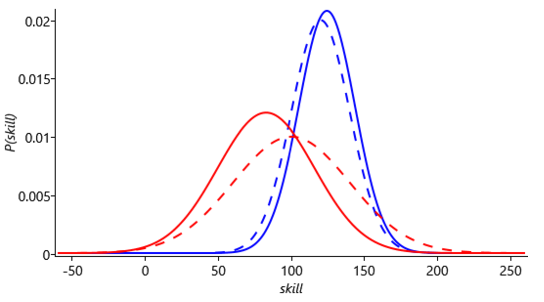
\includegraphics[scale=0.5]{black_predicted_wins}
    \caption{Black player wins, where black player is in blue and the white player is represented by the red curve. The priors are showed in dashed lines, whereas the posteriors are shown in solid lines~\cite{bishop2013model}.}
    \label{fig:black_predicted_wins}
\end{figure}

If, however, the black player loses, his skill becomes less than the one of the white player (in this concrete example). The white player's skill grows above the black player one, and significantly more than the white player's prior. This is illustrated in Figure~\ref{fig:black_loses}.

\begin{figure}[htpb!]
    \centering
    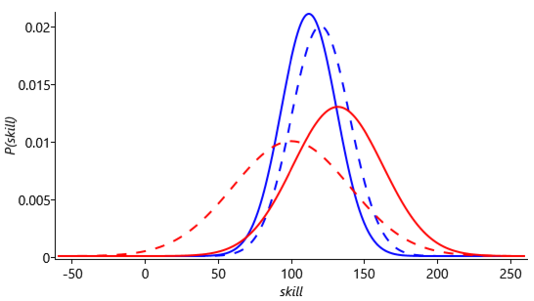
\includegraphics[scale=0.5]{black_loses}
    \caption{Black player loses, where black player is in blue and the white player is represented by the red curve. The priors are showed in dashed lines, whereas the posteriors are shown in solid lines~\cite{bishop2013model}.}
    \label{fig:black_loses}
\end{figure}


These posterior marginals (solid lines in Figure~\ref{fig:black_predicted_wins} and~\ref{fig:black_loses}) are an example of $p_a=\mathcal{N}(s;m;V)$ (dashed orange line in Figure~\ref{fig:diag_from_orig}).


\subsection{}
\label{sec:3c}

\begin{figure}[htpb!]
    \centering
    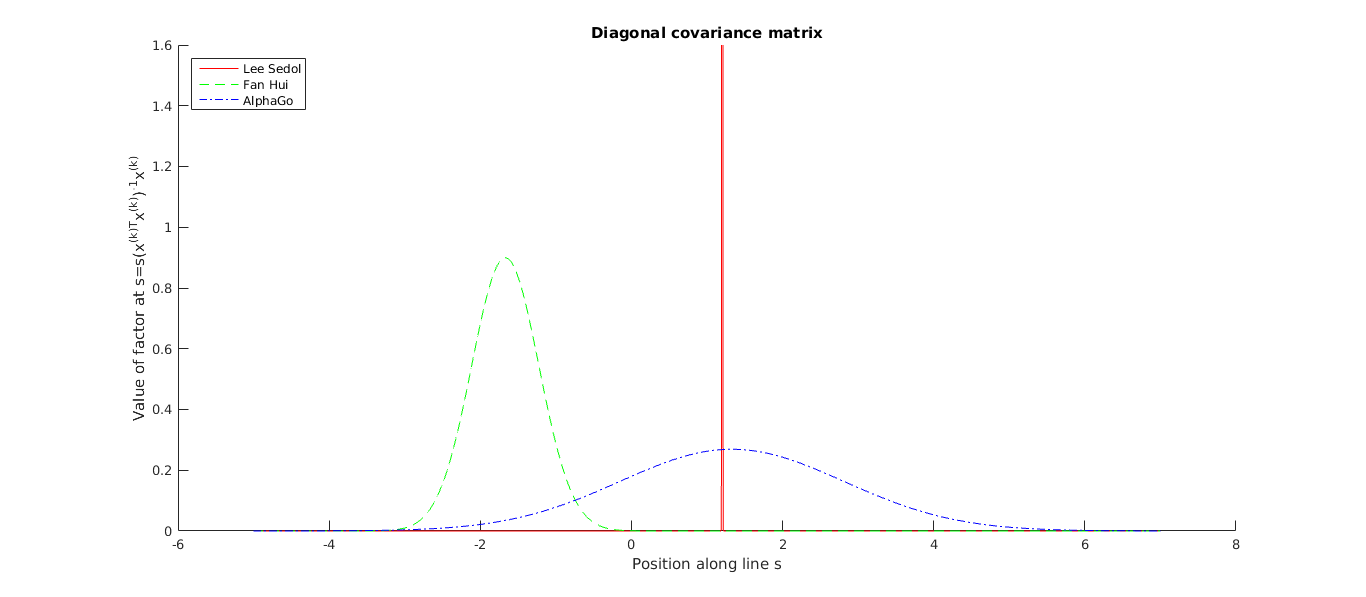
\includegraphics[scale=0.9]{3b_diag}
    \caption{Approximate posterior marginal distributions for AlphaGo, Fan Hui, Lee Sedol using diagonal covariance approximation.}
    \label{fig:3b_diag}
\end{figure}

\begin{figure}[htpb!]
    \centering
    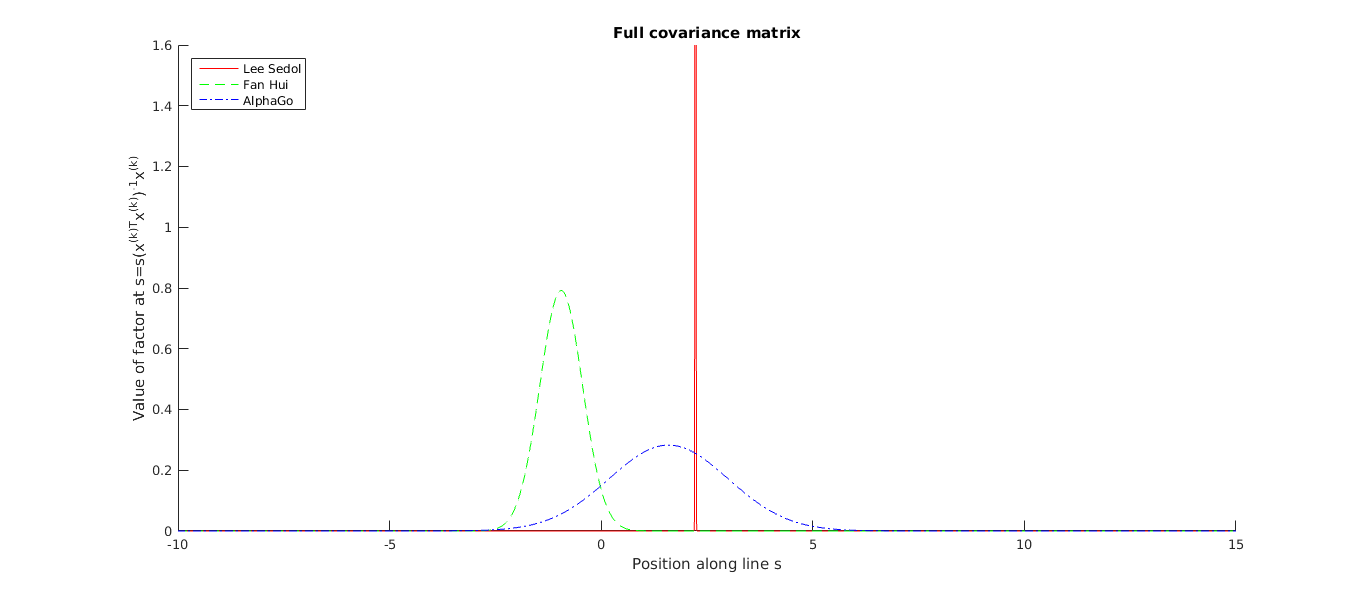
\includegraphics[scale=0.9]{3b_full}
    \caption{Approximate posterior marginal distributions for AlphaGo, Fan Hui, Lee Sedol using full covariance approximation.}
    \label{fig:3b_full}
\end{figure}

\begin{lstlisting}[label={list:3b},caption=Code for plotting approximate marginal posterior using full and diagonal approximations,language=MATLAB]
function [] = task3b()
%TASK3B Plots the approximate Gaussian posterior of each player with diagonal
%and full covariance matrices

    load('go_player_skill_model/diag_covar.mat');
    
    % set axis
    x = -5:.0012:7;
    
    figure(1);
    hold on;
    title('Diagonal covariance matrix');
    plot(x, normpdf(x, approx_mean(lee_sedol_id), approx_covar(lee_sedol_id)^0.5),'-r');
    plot(x, normpdf(x, approx_mean(fan_hui_id), approx_covar(fan_hui_id)^0.5),'--g');
    plot(x, normpdf(x, approx_mean(alpha_go_id), approx_covar(alpha_go_id)^0.5),'-.b');
    ylim([0 9]);
    legend('Lee Sedol','Fan Hui', 'AlphaGo', 'Location', 'northwest');
    xlabel('Skill');
    ylabel('P(Skill)');
    hold off;
    
    load('go_player_skill_model/full_covar.mat');
    
    figure(2);
    hold on;
    title('Full covariance matrix');
    plot(x, normpdf(x, approx_mean(lee_sedol_id), approx_covar(lee_sedol_id,lee_sedol_id)^0.5),'-r');
    plot(x, normpdf(x, approx_mean(fan_hui_id), approx_covar(fan_hui_id,fan_hui_id)^0.5),'--g');
    plot(x, normpdf(x, approx_mean(alpha_go_id), approx_covar(alpha_go_id,alpha_go_id)^0.5),'-.b');
    ylim([0 9]);
    legend('Lee Sedol','Fan Hui', 'AlphaGo', 'Location', 'northwest');
    xlabel('Skill');
    ylabel('P(Skill)');
    hold off;
    drawnow;
end

\end{lstlisting}

Distributions clearly show that the skill of the two "real" players - Lee Sedol and Fan Hui is well defined, as their variance using both full and diagonal approximation is way smaller, than the variance of AlphaGo. This can be explained by the fact that the two players have played more games than AlphaGo has.

Furthermore, it is interesting to see the difference between using the diagonal and full approximations with respect to the variance. For example, Fan Hui's variance when using the full approximation is larger than when using diagonal approximation. Same goes for Lee Sedol. Whereas, AlphaGo's variance behaves differently - it's lower for the full covariance matrix. Logically, this can be explained by the fact that the full covariance matrix contains more information, i.e. the covariance with respect to the other 1048 players, whereas the diagonal approximation only involves the variance. While this is partially true, there are more factors that have to be taken into account. Firstly, the full covariance matrix doesn't mean that each player played against each other, even though, the entries are non-zero. The reason for this is the inverse of the covariance matrix. Furthermore, the difference between the variance between Fan Hui and AlphaGo is very small, it can be considered as insignificant.

Finally, one can notice that there is a shift of the mean for all 3 players. When using the diagonal approximation one can see that Lee Sedol's and AlphaGo's skill mean are quite close, even though, their uncertainty level is very different. When using the full covariance matrix, however, we can clearly see, that Lee Sedol's skill is better defined in terms of the graph presented on Figure~\ref{fig:3b_full}. In addition, the skill mean of Lee Sedol is clearly above AlphaGo's one when using the full covariance matrix.

\subsection{}

\begin{equation}
    P(r=1|s_b=1049,s_w=26,approx=diag)=0.52726
    \label{eq:ag_vs_ls_diag}
\end{equation}

\begin{equation}
    P(r=1|s_b=1049,s_w=26,approx=full)=0.36533
    \label{eq:ag_vs_ls_full}
\end{equation}

\begin{lstlisting}[label={list:3c},caption=Code for computing the probability of AlphaGo winning when playing black against Lee Sedol using both full and diagonal covariance matrices.,language=MATLAB]
function [] = task3c()
%TASK3C Calculate the probability of AlphaGo winning, when playing as black
%using both diagonal and full covariance matrices

    format long
    
    load('go_player_skill_model/diag_covar.mat');
    
    % create your x vector to be a column vector with n_players size
    x = zeros(n_players, 1);
    
    % set Alpha Go with black
    x(alpha_go_id,1) = 1 / sqrt(2*performance_var);
    
    % set Lee Sedol with white
    x(lee_sedol_id,1) = -1 / sqrt(2*performance_var);
    
    numerator = approx_mean * x;
    
    denominator_diag = sqrt((x' * diag(approx_covar) * x) + 1);
    
    eq_diag = numerator / denominator_diag;
    
    disp(['P(r=1|s_b=',num2str(alpha_go_id), ',s_w=',num2str(lee_sedol_id),',approx=diag)=',num2str(normcdf(eq_diag))]);
    
    load('go_player_skill_model/full_covar.mat');
    
    numerator_full = approx_mean * x;
    
    denominator_full = sqrt((x' * approx_covar * x) + 1);
    
    eq_full = numerator_full / denominator_full;
    
    disp(['P(r=1|s_b=',num2str(alpha_go_id), ',s_w=',num2str(lee_sedol_id),',approx=full)=',num2str(normcdf(eq_full))]);
    
end
\end{lstlisting}

\subsection{}
Considering the two results in Equation~\ref{eq:ag_vs_ls_diag} and~\ref{eq:ag_vs_ls_full}, as well as the two graphs in Figure~\ref{fig:3b_full} and~\ref{fig:3b_diag}, one could argue that the results are expected. Meaning that when using the diagonal covariance matrix, where the mean of Lee Sedol and Alpha Go is quite close, AlphaGo has 52.726\% of winning. When using the full covariance matrix, one could also observe that as the distributions are further apart, with Lee Sedol's PDF having advantage, it is reasonable to assume that AlphaGo has a lower chance of winning - 36.533\%.

However, as previously mentioned in Section~\ref{sec:3c}, the full covariance matrix is more informative, as it has the covariances between the rest of the players. In other words it takes into account the previously played games between players when computing the marginal posterior. Having said that, the accuracy of the estimated posterior might be hard to evaluate. The reason is that the skill of a player is something not actually observable, but can be regarded as hidden variable. Thus, it would take lots of trial and error in order to determine whether the approximation is correct or not. These experiments would have to be based on observations of game outcomes.
This can be confirmed by the fact that on both Figure~\ref{fig:diag_from_orig} and~\ref{fig:full_from_orig} the diagonal and full covariance matrix approximate the true factor almost identically.

\begin{figure}[htpb!]
    \centering
    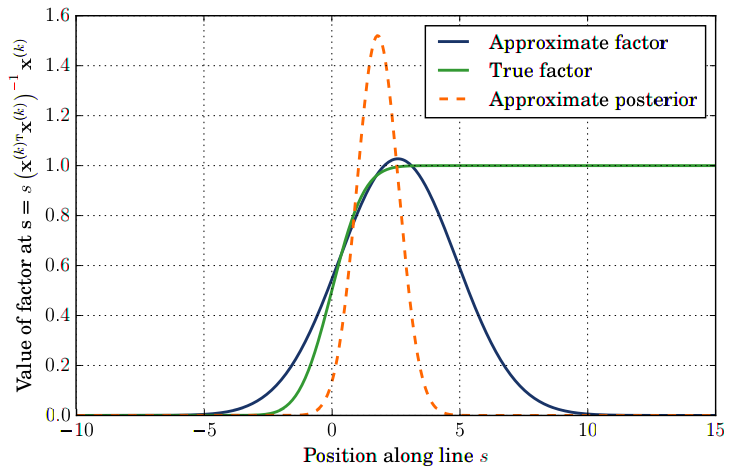
\includegraphics[scale=0.5]{full_from_ass}
    \caption{Values of corresponding approximate and true factors and scaled value of approximate posterior density along line $s=s|x^{(k)}|^{-1}x^{(k)}$ for a single factor in the full covariance approximate densities.}
    \label{fig:full_from_orig}
\end{figure}

On the other hand, if we have to consider millions of Go players, then the full matrix computation will become very inefficient, as it is computationally expensive to inverse the full covariance matrix. Whereas, inversing the main diagonal of a matrix is essentially inversing a vector, which will take linear time. In fact, Sch{\"o}lkopf et al argue that adopting the full covariance approximation approach, an extra complexity of $\mathcal{O}(K^3N^3)$ is added~\cite{scholkopf2007advances}. Furthermore, they show that when using the diagonal matrix, we lose the "explicit posterior coupling"~\cite{scholkopf2007advances}.

\section{}

\subsection{}
As shown in Section~\ref{sec:2f}, when computing the Cumulative Density Function, the model considers only the pure skill of the player. A possible extension of the model would be to add an additional constant that would account for the disadvantage of playing with the white stones. This extension, $komi$, however, needs to be weighted, based on the difference in the skills of the two players. For example, consider two games, in the first one $s_w^1$ plays $s_b^2$, and the difference between them is 2000, and in the second game $s_b^1$ plays $s_w^3$, where the skill difference is only 10. If a constant $komi$ is added to the CDF calculation, then it might result in very different approximations. This weighted factor, by which the $komi$ should be weighted might be hard to compute, as it would involve numerous observations of game outcomes. Mathematically this extension can be expressed as follows:

\begin{equation}
    \Phi \Big[ \frac{s_b - s_w}{\sqrt{2}\beta} + \frac{K}{K_{factor}} \Big]
\end{equation}

A similar implementation was considered in~\cite{stanescu2011rating}, with the slight difference of accounting for handicapped games. In my opinion, accounting for the extension would shift the approximation of the CDF towards the skill of the white player, in order to compensate for the advantage of starting first. This will eventually result in more accurate calculations of the approximate posteriors for the skills of both players.

\subsection{}
In the model so far, we have assumed that the player skill will be fixed, even though we are trying to approximate it, we do not allow it to change dynamically over time. Such situations might happen, when for example, a player has a "bad" day, when he is not performing up to his usual standards, for instance. In order to model this, we can extend the model to account for skill at any given time $t \in \{1..T\}$, such that, $p(s^t|s^{t-1})=\mathcal{N}(0, s_{change})$. In other words, the skill changes through time, where that change is modelled with a zero-mean Gaussian. This means that the skill varies from game to game and on average it does not vary much, i.e. $\mu_{change}=0$. Therefore, our skill posterior will be updated as follows~\cite{bishop2013model}:

\begin{equation}
    \label{eq:4b_bishop}
    s^t = s^{t-1}+s_{change} = \mathcal{N}(s^t;\mu_{s^{t-e}}, \Var(s_{change}))
\end{equation}

Therefore, the updated factor graph for 2 consecutive games between 2 paired players would look like so:

\begin{figure}[htpb!]
    \centering
    \tikz{ %
        \node[obs] (r1) {$r^{(1)}$} ; %
        \node[latent, left=of r1, yshift=0.9cm, xshift=-0.7cm] (pw) {$p^{t-1}_w$} ; %
        \node[latent, left=of r1, below=of pw] (pb) {$p^{t-1}_b$} ; %
        \factor[left=of r1, xshift=-0.2cm] {r1-factor} {} {} {};
        \edge {pw,pb} {r1-factor} ; %
        \edge {r1-factor} {r1}; %
        \factor[left=of pw, xshift=-.6cm] {pw-factor} {below:$\mathcal{N}(p^{t-1}_w;s^{t-1}_w,\beta^2)$} {} {};
        \factor[left=of pb, xshift=-.6cm] {pb-factor} {above:$\mathcal{N}(p^{t-1}_b;s^{t-1}_b,\beta^2)$} {} {};
        \node[latent, left=of pw, xshift=-1.2cm] (sw) {$s^{t-1}_w$} ; %
        \node[latent, left=of pb, xshift=-1.2cm] (sb) {$s^{t-1}_b$} ; %
        \edge {sw} {pw-factor} ; %
        \edge {sb} {pb-factor} ; %
        \edge {pw-factor} {pw} ; %
        \edge {pb-factor} {pb} ; %
        \factor[left=of sw, xshift=-1.2cm] {sw-factor} {left:$\mathcal{N}(s^{t-1}_w;0,\sigma^2)$} {} {};
        \factor[left=of sb, xshift=-1.2cm] {sb-factor} {left:$\mathcal{N}(s^{t-1}_b;0,\sigma^2)$} {} {};
        \edge {sw-factor} {sw} ; %
        \edge {sb-factor} {sb} ; %
        \node[const, left=of r1-factor, xshift=-3cm]  (beta) {$\beta$} ; %
        \node[const, left=of beta, xshift=-2cm]  (alpha) {$\alpha$} ; %
        \edge[dotted] {beta} {pb-factor} ; %
        \edge[dotted] {beta} {pw-factor} ; %
        \edge[dotted] {alpha} {sb-factor} ; %
        \edge[dotted] {alpha} {sw-factor} ; %
        %\draw node [above=of alpha, fill=white, xshift=2cm] {\textcolor{red}{(1)}};
        %\draw node [above=of alpha, fill=white, xshift=3.9cm] {\textcolor{red}{(2)}};
        %\draw node [above=of alpha, fill=white, xshift=5.1cm] {\textcolor{red}{(3)}};
        %\draw node [above=of alpha, fill=white, xshift=7cm, yshift=-0.5cm] {\textcolor{red}{(4)}};
        %\draw node [above=of alpha, fill=white, xshift=7.7cm, yshift=-1cm] {\textcolor{red}{(5)}};
        %\draw node [above=of alpha, fill=white, xshift=7cm, yshift=-2.3cm] {\textcolor{blue}{(6)}};
        %\draw node [above=of alpha, fill=white, xshift=5.1cm, yshift=-2.7cm] {\textcolor{blue}{(7)}};
        %\draw node [above=of alpha, fill=white, xshift=3.9cm, yshift=-2.7cm] {\textcolor{blue}{(8)}};
        %\draw node [above=of alpha, fill=white, xshift=2cm, yshift=-2.7cm] {\textcolor{red}{(9)}};
        
        % second game
        \node[obs, below=of r1, yshift=-2cm] (r2) {$r^{(2)}$} ; %
        \node[latent, left=of r2, yshift=0.9cm, xshift=-0.7cm] (pw2) {$p^{t}_w$} ; %
        \node[latent, left=of r2, below=of pw2] (pb2) {$p^{t}_b$} ; %
        \factor[left=of r2, xshift=-0.2cm] {r2-factor} {} {} {};
        \edge {pw2,pb2} {r2-factor} ; %
        \edge {r2-factor} {r2}; %
        \factor[left=of pw2, xshift=-.6cm] {pw2-factor} {below:$\mathcal{N}(p^t_w;s^t_w,\beta^2)$} {} {};
        \factor[left=of pb2, xshift=-.6cm] {pb2-factor} {above:$\mathcal{N}(p^t_b;s^t_b,\beta^2)$} {} {};
        \node[latent, left=of pw2, xshift=-1.2cm] (sw2) {$s^{t-1}_w$} ; %
        \node[latent, left=of pb2, xshift=-1.2cm] (sb2) {$s^{t-1}_b$} ; %
        \edge {sw2} {pw2-factor} ; %
        \edge {sb2} {pb2-factor} ; %
        \edge {pw2-factor} {pw2} ; %
        \edge {pb2-factor} {pb2} ; %
        \factor[left=of sw2, xshift=-1.2cm, yshift=1cm] {sw2-factor} {left:$\mathcal{N}(s^t_w;0,s^2_{change})$} {} {};
        \factor[left=of sb2, xshift=-1.2cm, yshift=1cm] {sb2-factor} {left:$\mathcal{N}(s^t_b;0,s^2_{change})$} {} {};
        \edge[color=blue] {sw} {sw2-factor} ; %
        \edge[color=blue] {sb} {sb2-factor} ; %
        \edge[color=blue] {sw2-factor} {sw2}; %
        \edge[color=blue] {sb2-factor} {sb2}; %
        \node[const, left=of r2-factor, xshift=-3cm]  (beta2) {$\beta$} ; %
        \edge[dotted] {beta2} {pb2-factor} ; %
        \edge[dotted] {beta2} {pw2-factor} ; %
        \edge[dotted] {alpha} {sw-factor} ; %
    }
    \caption{Factor graph of Gaussian player skill model for a two consecutive games between 2 paired players. The variables used are similar to the ones in Figure~\ref{fig:fig_2_assignment}, with the difference of the time step $t \in \{1..T\}$. In addition the figure presents a model that accounts for the change of skill between games by introducing a two new factors ($\mathcal{N}(s^t_w;0,s^2_{change})$ and $\mathcal{N}(s^t_b;0,s^2_{change})$). They act as the new prior in the following game, introducing more uncertainty between games.}
    \label{fig:skill_var_time}
\end{figure}

In~\cite{bishop2013model}, Winn and Bishop suggest that we firstly run expectation propagation in the game with outcome $r^{(1)}$. Then, the outgoing messages, from $s^{t-1}_w$ and $s^{t-1}_w$ to $s^{t}_w$ and $s^{t}_w$, are updated skill distributions that pass through the new Gaussian Factors. However, when convoluting these messages with the Gaussian factor (for example $\mathcal{N}(s^t_w;0,s^2_{change})$), essentially, we are introducing more uncertainty between games. This convolution is then used as the new prior for the next game. While introducing more uncertainty with every game may not be intuitive, it allows us to model the skill change of a player through time. Essentially, this new model allows to reflect the possibility of a change in players' skill.

Figure~\ref{fig:mbml_dynamic_skill_update} shows the improvement made by Winn and Bishop using this model over the previous one. The red line denotes the true skill change, the blue line shows the inferred skill change under the original model used in Section~\ref{sec:2} and~\ref{sec:3}. The green curve shows the updated model's inference, supporting the change of skill over time.

\begin{figure}[htpb!]
    \centering
    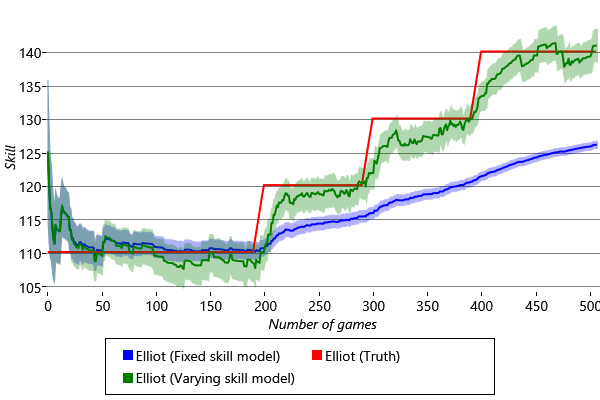
\includegraphics[scale=1]{TrueSkill_DynamicsDemo_Trajectories[2]}
    \caption{Figure adopted from~\cite{bishop2013model}. Elliot is the player who skill is being modelled. Red line denotes the true skill change, blue line shows the inferred skill change under the original model (Figure~\ref{fig:fig_2_assignment}), green curve shows the updated model's inference, supporting the change of skill over time.}
    \label{fig:mbml_dynamic_skill_update}
\end{figure}

This approach has several drawbacks - it depends on the order of the update, as well as it does not account for the very old games~\cite{dangauthier2007trueskill}. For instance, on Figure~\ref{fig:mbml_dynamic_skill_update}, if the first 200 games are played 2 years ago, then the model might not be relevant, as other factors could potentially influence players' skill. The second drawback is that inference is only propagated forward in time~\cite{dangauthier2007trueskill}. For example, if player A plays an unseen opponent B and wins, but this opponent turns out to be very good, then the skill of player A is not properly adjusted.

An alternative, suggested by Dangauthier et al is to use a method called TrueSkill Through Time (TTT)~\cite{dangauthier2007trueskill}. Their improvement can be partially applied to the aforementioned model. A significant change would be to track the game outcomes based on different years. For example, $r^{(1)}$ and $r^{(2)}$ will become $r^{y(1)}$ and $r^{y(2)}$ to relate them to games in the same time period (years in this case). This is described as the Vanilla TrueSkill in~\cite{dangauthier2007trueskill}. In order to improve this Vanilla TrueSkill, we have to run the full EP algorithm until convergence for a certain time period ($y$). An important note is that the previous update of the result of a game must be removed before the new one is applied. Thus, the model is consistent, but less approximate~\cite{dangauthier2007trueskill}.

\subsection{WRITEMEWRITEMEWRITEMEWRITEMEWRITEMEWRITEMEWRITEMEWRITEMEWRITEMEWRITEMEWRITEMEWRITEMEWRITEMEWRITEMEWRITEMEWRITEMEWRITEMEWRITEMEWRITEMEWRITEMEWRITEMEWRITEMEWRITEMEWRITEMEWRITEMEWRITEMEWRITEMEWRITEMEWRITEMEWRITEME}
In Section~\ref{sec:3}, the expectation propagation inference method is used, that allow intractable distributions to be approximated by Gaussians, it is considered to be the generalisation of loopy belief propagation. In Section~\ref{sec:3}, it is shown how from a normal CDF, we can approximate a Gaussian distribution and use that instead, in order to have a conjugate prior - Gaussian.

A clear disadvantage of EP is that it might not converge~\ref{bishop2006pattern}. However, this is not the case for our model, thus it will not be discussed in detail. Another drawback of EP is that

when evaluating the big integral, the first term is relatively easy to compute, whereas the second term could be very computationally expensive. Thus, one could use the alternative of Gibbs sampling for that case.

Alternatively, one could use variational approximation 

Note that we can compute r|sb,sw easily, but we can use gibbs sampling for the other term.

\clearpage

\bibliographystyle{plain}
\bibliography{bibliography}
\clearpage

\end{document}

